	\section{Arbre de Régréssion et Forêt Aléatoire}
\label{section:RF}
\subsection{Bagging}
Le \textit{bagging}, ou \textit{bootstrap aggregrating} est un ensemble de méthodes d'apprentissage qui combinent différents estimateurs entraînés sur des échantillons \textit{bootstrap} \footnote{Tirage aléatoire avec remise}. Une \textit{forêt aléatoire} est une méthode de bagging consistant à entraîner un ensemble de $B$ arbres de classification ou de régression (Classification And Regression Trees, CART) et à prédire la moyenne des prédictions des $B$ arbres.

\subsection{Arbres de classification et de régression (CART)}
\label{subsection:CART}
Un Arbre de Classification ou de Régression (Classification And Regression Trees, CART) \cite{breiman1984classification} est construit par partitionnement binaire récursif de l'espace des variables explicatives (voir figure \ref{fig:partitioncart}). À chaque nœud, l'algorithme sélectionne la variable et le seuil de coupure qui minimisent le plus la variance intra-groupe des sous-ensembles résultants. Ce processus est répété récursivement jusqu'à ce qu'un critère d'arrêt soit atteint. La prédiction d'une nouvelle observation correspond, dans le cas d'une régression, à la moyenne des valeurs observées dans la feuille terminale où elle est routée.

\begin{figure}[H]
	\centering
	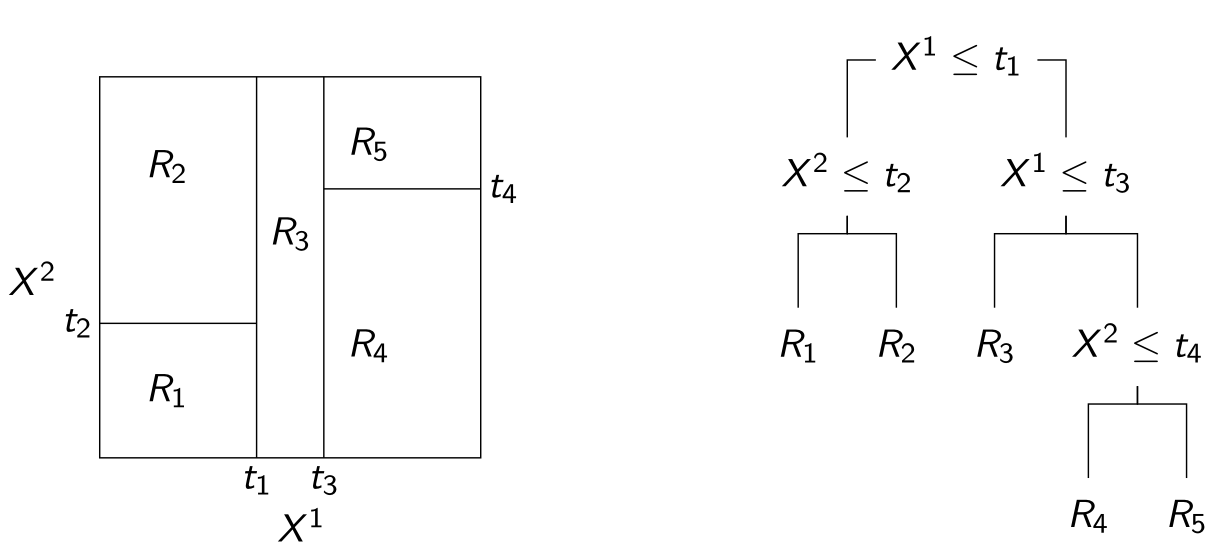
\includegraphics[width=0.8\linewidth]{images/03_methode/partition_cart}
	\caption{Schéma du partitionnement de l'espace des covariable par CART \cite{fischer2026}.}
	\label{fig:partitioncart}
\end{figure}

De manière plus formelle, on dispose d'un échantillon $\mathcal{D}_n = \{(X_1,Y_1),\dots,(X_n,Y_n)\}$ de couples indépendants et de même loi que $(X,Y)$, où $X = (X^{(1)},\dots,X^{(d)}) \in \mathbb{R}^d$ et $Y \in \mathbb{R}$. L'objectif est d'estimer la fonction de régression $f(x) = \mathbb{E}[Y \mid X = x]$. \\

\paragraph{Partitionnement et critère de coupure}
Un arbre partitionne récursivement l'espace des variables $\mathbb{R}^d$ en rectangles, chaque rectangle correspondant à un noeud de l'arbre. Soit $\mathcal{D}$ l'échantillon utilisé pour construire l'arbre, $R \subseteq \mathbb{R}^d$ un noeud et $n_R = \sum_{i}^n \mathds{1}_{\{X_i \in R\}}$ le nombre d'observations de $\mathcal{D}$ qui tombent dans $R$.\\

Une coupure est un couple $(j,t) \in \{1,\dots,d\} \times \mathbb{R}$, avec $j \in d$ la variable et $t \in \mathbb{R}$ le seuil de coupure. Elle partitionne le noeud $R$ en deux noeuds fils $R_1 (j,t)$ et $R_2(j,t)$ :
\[
R_1(j,t) = \{x \in R : x_j < t\}
\qquad\text{et}\qquad
R_2(j,t) = \{x \in R : x_j \ge t\},
\]
d'effectifs respectifs $n_1(j,t) = n_{R_1(j,t)}$ et $n_2(j,t) = n_{R_2(j,t)}$, avec $n_1(j,t) + n_2(j,t) = n_R$. 


On souhaite trouver une manière de partitionner les variables telle que les deux nouvelles régions $R_1 (j, t)$ et $R_2(j, t)$ issues de cette partition soient les plus homogènes possibles. Cela revient à, dans le cas de la régression, minimiser la variance de chaque noeud $R$ (critère d'impureté) :

\begin{equation}\label{eq:variance}
	V(R) = \frac{1}{n_R} \sum_{i : X_i \in R} \bigl(Y_i - \overline{Y}_R\bigr)^2
	\qquad\text{où}\qquad
	\overline{Y}_R = \frac{1}{n_R} \sum_{i : X_i \in R} Y_i .
\end{equation}

La qualité d'une coupure $(j,t)$ admissible est mesurée par la diminution d'impureté qu'elle produit, ou gain d'information (Information Gain, IG) :
\begin{equation}\label{eq:gain}
	\text{IG}_R(j,t) = V(R)
	- \frac{n_1(j,t)}{n_R}\, V\bigl(R_1(j,t)\bigr)
	- \frac{n_2(j,t)}{n_R}\, V\bigl(R_2(j,t)\bigr).
\end{equation}

Les variances des fils sont pondérées par la proportion d'observations qu'ils
contiennent, de sorte que $	\text{IG}_R(j,t) \ge 0$ (décomposition de la variance
totale en variances intra- et inter-groupes). La meilleure coupure parmi un
ensemble de variables candidates $\mathcal{M} \subseteq \{1,\dots,d\}$ est
\begin{equation}\label{eq:meilleure}
	(j^\star, t^\star) \in
	\text{argmax}_{j \in \mathcal{M},\; t \in \mathcal{T}_j(R)} 	\text{IG}_R(j,t).
\end{equation}

\paragraph{Prédiction d'un arbre}

Pour $x \in \mathbb{R}^d$, on note $R(x)$ la feuille de l'arbre $\hat f$ contenant $x$ et $n_{R(x)}$ le nombre de points de $\mathcal{D}_m$  qui y tombent. La prédiction de
l'arbre est la moyenne des réponses de cette feuille :
\begin{equation}
	\label{eq:arbre}
	\hat f(x) = \overline{Y}_{R(x)}
	= \frac{1}{n_{R(x)}}
	\sum_{(X_i,Y_i) \in \mathcal{D}_m} Y_i \, \mathds{1}_{\{X_i \in R(x)\}}
\end{equation}

\subsection{Forêt Aléatoire} 
\label{subsection:RF}
Une forêt aléatoire \cite{breiman2001} est une méthode de bagging consistant à tirer $B$ échantillons bootstrap à partir de $\mathcal{D}_n$, puis construire un arbre CART sur chacun d'eux et enfin agréger les prédictions des $B$ arbres. Les CART construits sont cependant légèremment différents : à chaque noeud, la meilleure coupure n'est pas cherchée parmi les $d$ variables, mais parmi un sous-ensemble de $p \le d$ variables tirées au hasard.

\paragraph{Construction de la forêt}
Pour $b = 1, \dots, B$, on tire avec remise un échantillon bootstrap $\mathcal{D}_m^{(b)}$ de taille $m$ dans $\mathcal{D}_n$, puis on construit un arbre $\hat f^{(b)}$ sur $\mathcal{D}_m^{(b)}$ par partitionnement récursif. À chaque noeud $R$, on tire uniformément et sans remise un ensemble $\mathcal{M} \subseteq \{1,\dots,d\}$ de $p$ variables, et on coupe $R$ selon la coupure $(j^\star, t^\star)$ définie par \eqref{eq:meilleure}. Le tirage de $\mathcal{M}$ est effectué indépendamment à chaque noeud. 

\paragraph{Prédiction de la forêt}
Pour chaque arbre $b \in [1, \ldots, B]$, la prédiction $\hat f^{(b)}(x)$ est donnée par \eqref{eq:arbre} (en remplaçant $\mathcal{D}_m$ par $\mathcal{D}_m^{(b)}$). La forêt prédit la moyenne des $B$ arbres :
\begin{equation}\label{eq:foret}
	\hat f_B(x) = \frac{1}{B} \sum_{b=1}^{B} \hat f^{(b)}(x).
\end{equation}

\paragraph{Hyperparamètres}
La construction de forêts aléatoires dépend donc de quatre hyperparamètres : 
\begin{itemize}
	\item $B$ le nombre d'arbres (\texttt{num.trees}),
	\item $m$ la taille des échantillons bootstrap (\texttt{sample.fraction}),
	\item $p$ le nombre de variables candidates pour chaque split (\texttt{mtry}),
	\item $n_{\min}$ l'effectif minimal des feuilles (\texttt{min.node.size})
\end{itemize}  